\section{Schaltplan}

\begin{figure}
	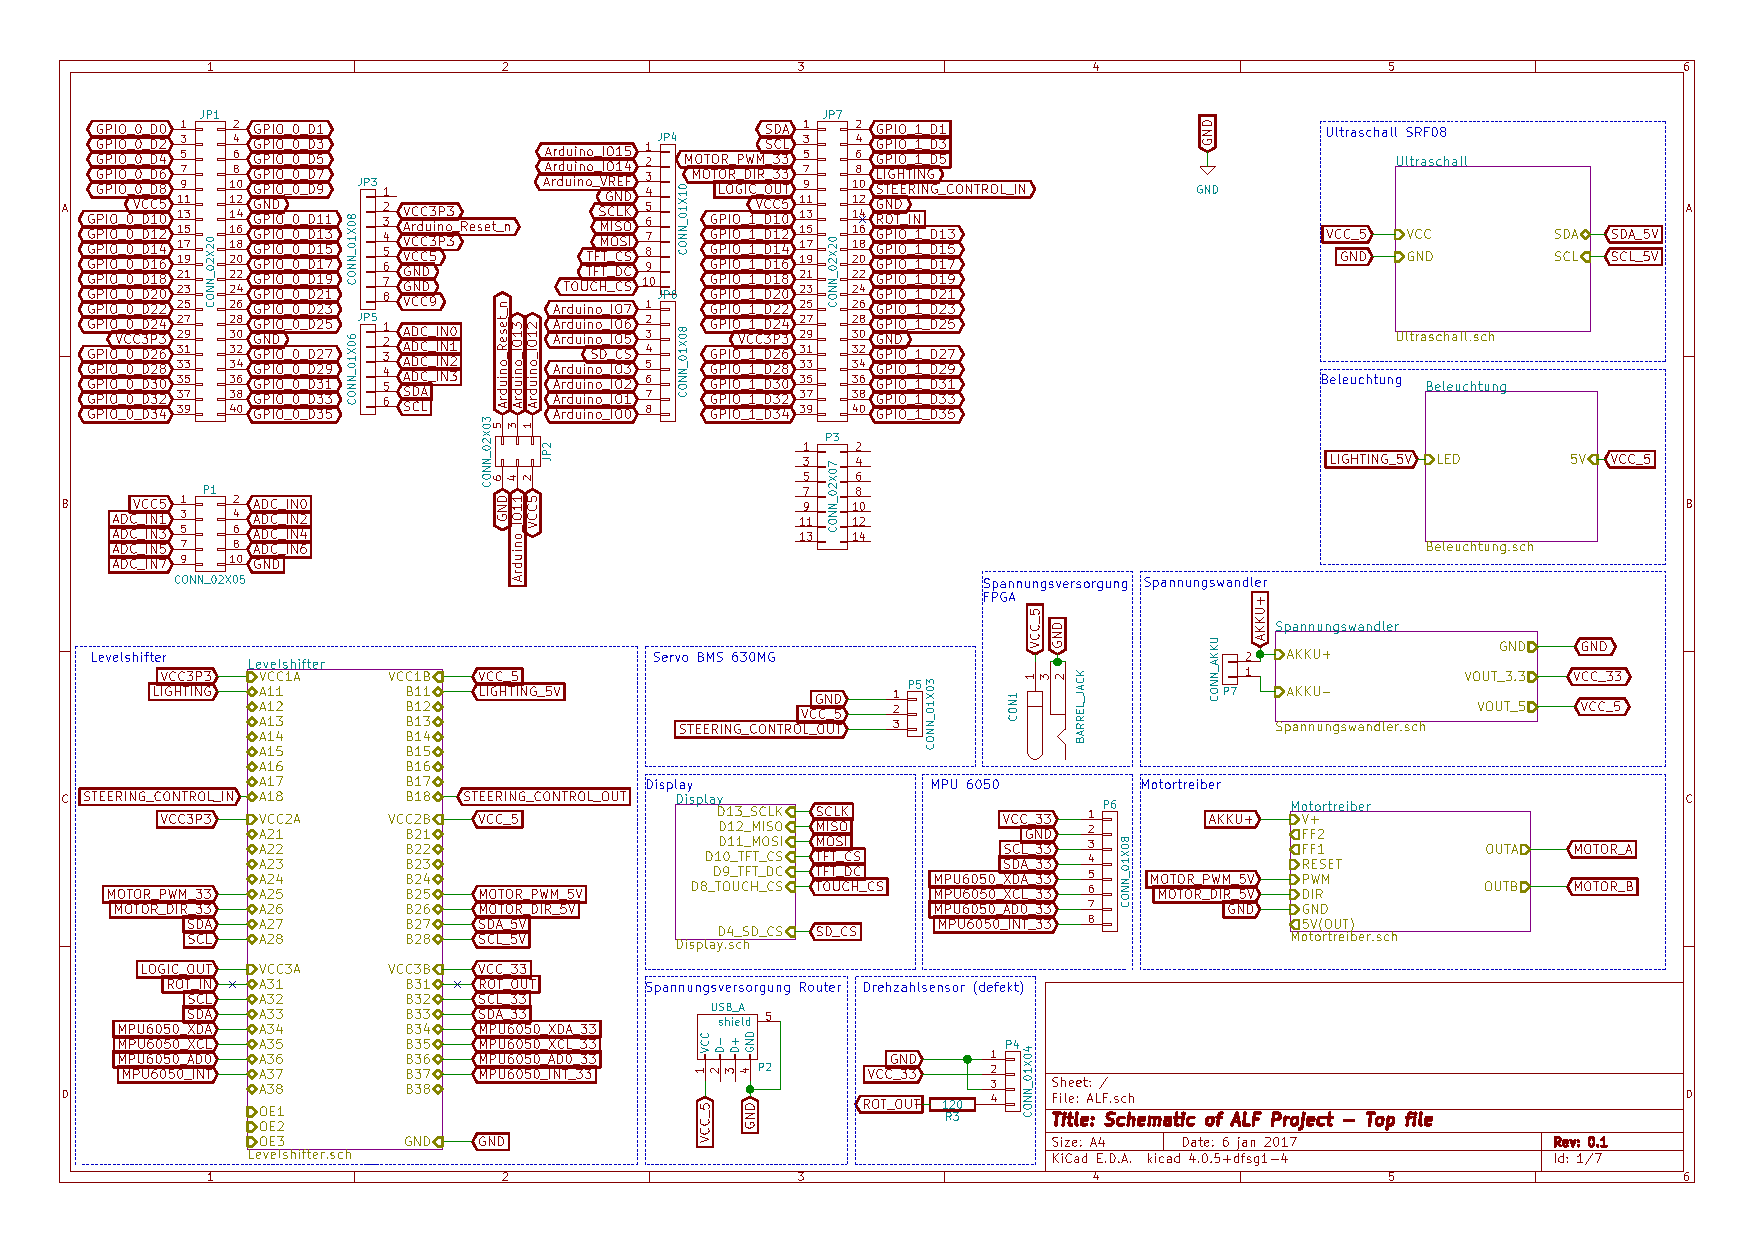
\includegraphics[angle=90, height=\textheight]{Abb/Garfield_Circuit.pdf}
	\caption{Schaltplan mit FPGA und verwendeter Peripherie}
	\label{Garfield_Circuit}
\end{figure}
Abbildung \ref{Garfield_Circuit} zeigt den erstellten Schaltplan des HSP. Dieser soll nachfolgend kurz beschrieben werden.\\
Alle ein- und ausgeheneden Signale mit Ausnahme der SPI Pins zur Ansteuerung des Displays (vgl. Abb. \ref{Garfield_Circuit} JP4) werden über Levelshifter geführt. Dies ermöglicht es zum einen alle Signale an die jeweils notwendigen Pegel anzupassen und zum anderen den maximalen vom FPGA bereitgestellten Strom nicht zu überschreiten. Dadurch ergeben sich die zwei Logikpegel 3,3V und 5V im System. Über den IIC Port werden alle Ultraschallsensoren und die MPU6050 angesprochen. Es wurden die internen pull-up Widerstände des IIC Ports aktiviert um dessen Funktionsfähigkeit sicherzustellen. Über den PWM Generator wird die Lenkung und der Motortreiber für die Geradeausfahrt angesteuert. Zur Ansteuerung der Beleuchtung und dem Setzen der Richtung des Motors werden einfache GPIO Pins benutzt. Der Schaltplan enthält zudem die Ansteuerung des Rotary Encoders zum Messen der Drehzahl des Motors. Da dieser jedoch unerwarteterweise nicht funktionsfähig war, sind die betrefenden Stellen im Schaltplan entsprechend gekennzeichnet.
\section{\ac{FPGA} Design}
Die Beschreibung des \ac{FPGA} wird, soweit möglich, mit dem Systemintegrationstool QSYS, das Teil der Quartus Toolchain ist, durchgeführt. Das Mapping zwischen QSYS-System und Pins wird klassisch in VHDL beschrieben. Das Top-Level-File des Systems ist \\ \texttt{FPGA\_Design/Garfield\_Design/Garfield.vhdl}. Dort wird das von QSYS erzeugt System und einige kleine \ac{IP}-Cores zusammengeführt und auf definierte Aus-/Eingänge geführt. Diese Ein-/Ausgänge werden dann über den \textit{Pin-Planner} auf die physikalischen Pins geführt.\\
Im Projektverzeichnis befinden sich alle Dateien, die für den \ac{FPGA} Teil relevant sind, unter \texttt{FPGA\_Design}. Die Struktur ab diesem Ordner ist wie folgt aufgebaut:
\begin{itemize}
	\item \texttt{Datasheets} - Einie Datenblätter und Application Notes zu dem \ac{FPGA} Teilprojekt
	\item \texttt{Garfield\_Design} - In diesem Ordner befinden sich die Quartus Projektdateien, Konfigurationsdateien und das QSYS Projekt.
	\item \texttt{ip\_extern} - Eine Sammlung von externen \ac{IP}-Cores, die im Projekt verwendet wurden. Es befinden sich dort nur die \ac{IP}-Cores, die nicht von Altera stammen oder nicht direkt in QSYS verfügbar sind.
	\item \texttt{ip\_intern} - Alle \ac{IP}-Cores, die für dieses Projekt entwickelt wurden.
	\item \texttt{output\_files} - In jedem Unterordner innerhalb dieses Ordners befinden sich \ac{FPGA} Images und die entsprechenden Konfigurationsdateien um ein Softwareprojekt dafür zu bauen.
\end{itemize}

Im folgenden werden die alle Systemkomponenten, die für das \Projectname-Projekt erzeugt wurden, beschrieben.

\section{\ac{IP}-Cores}
\label{IP-Cores}

\begin{figure}
	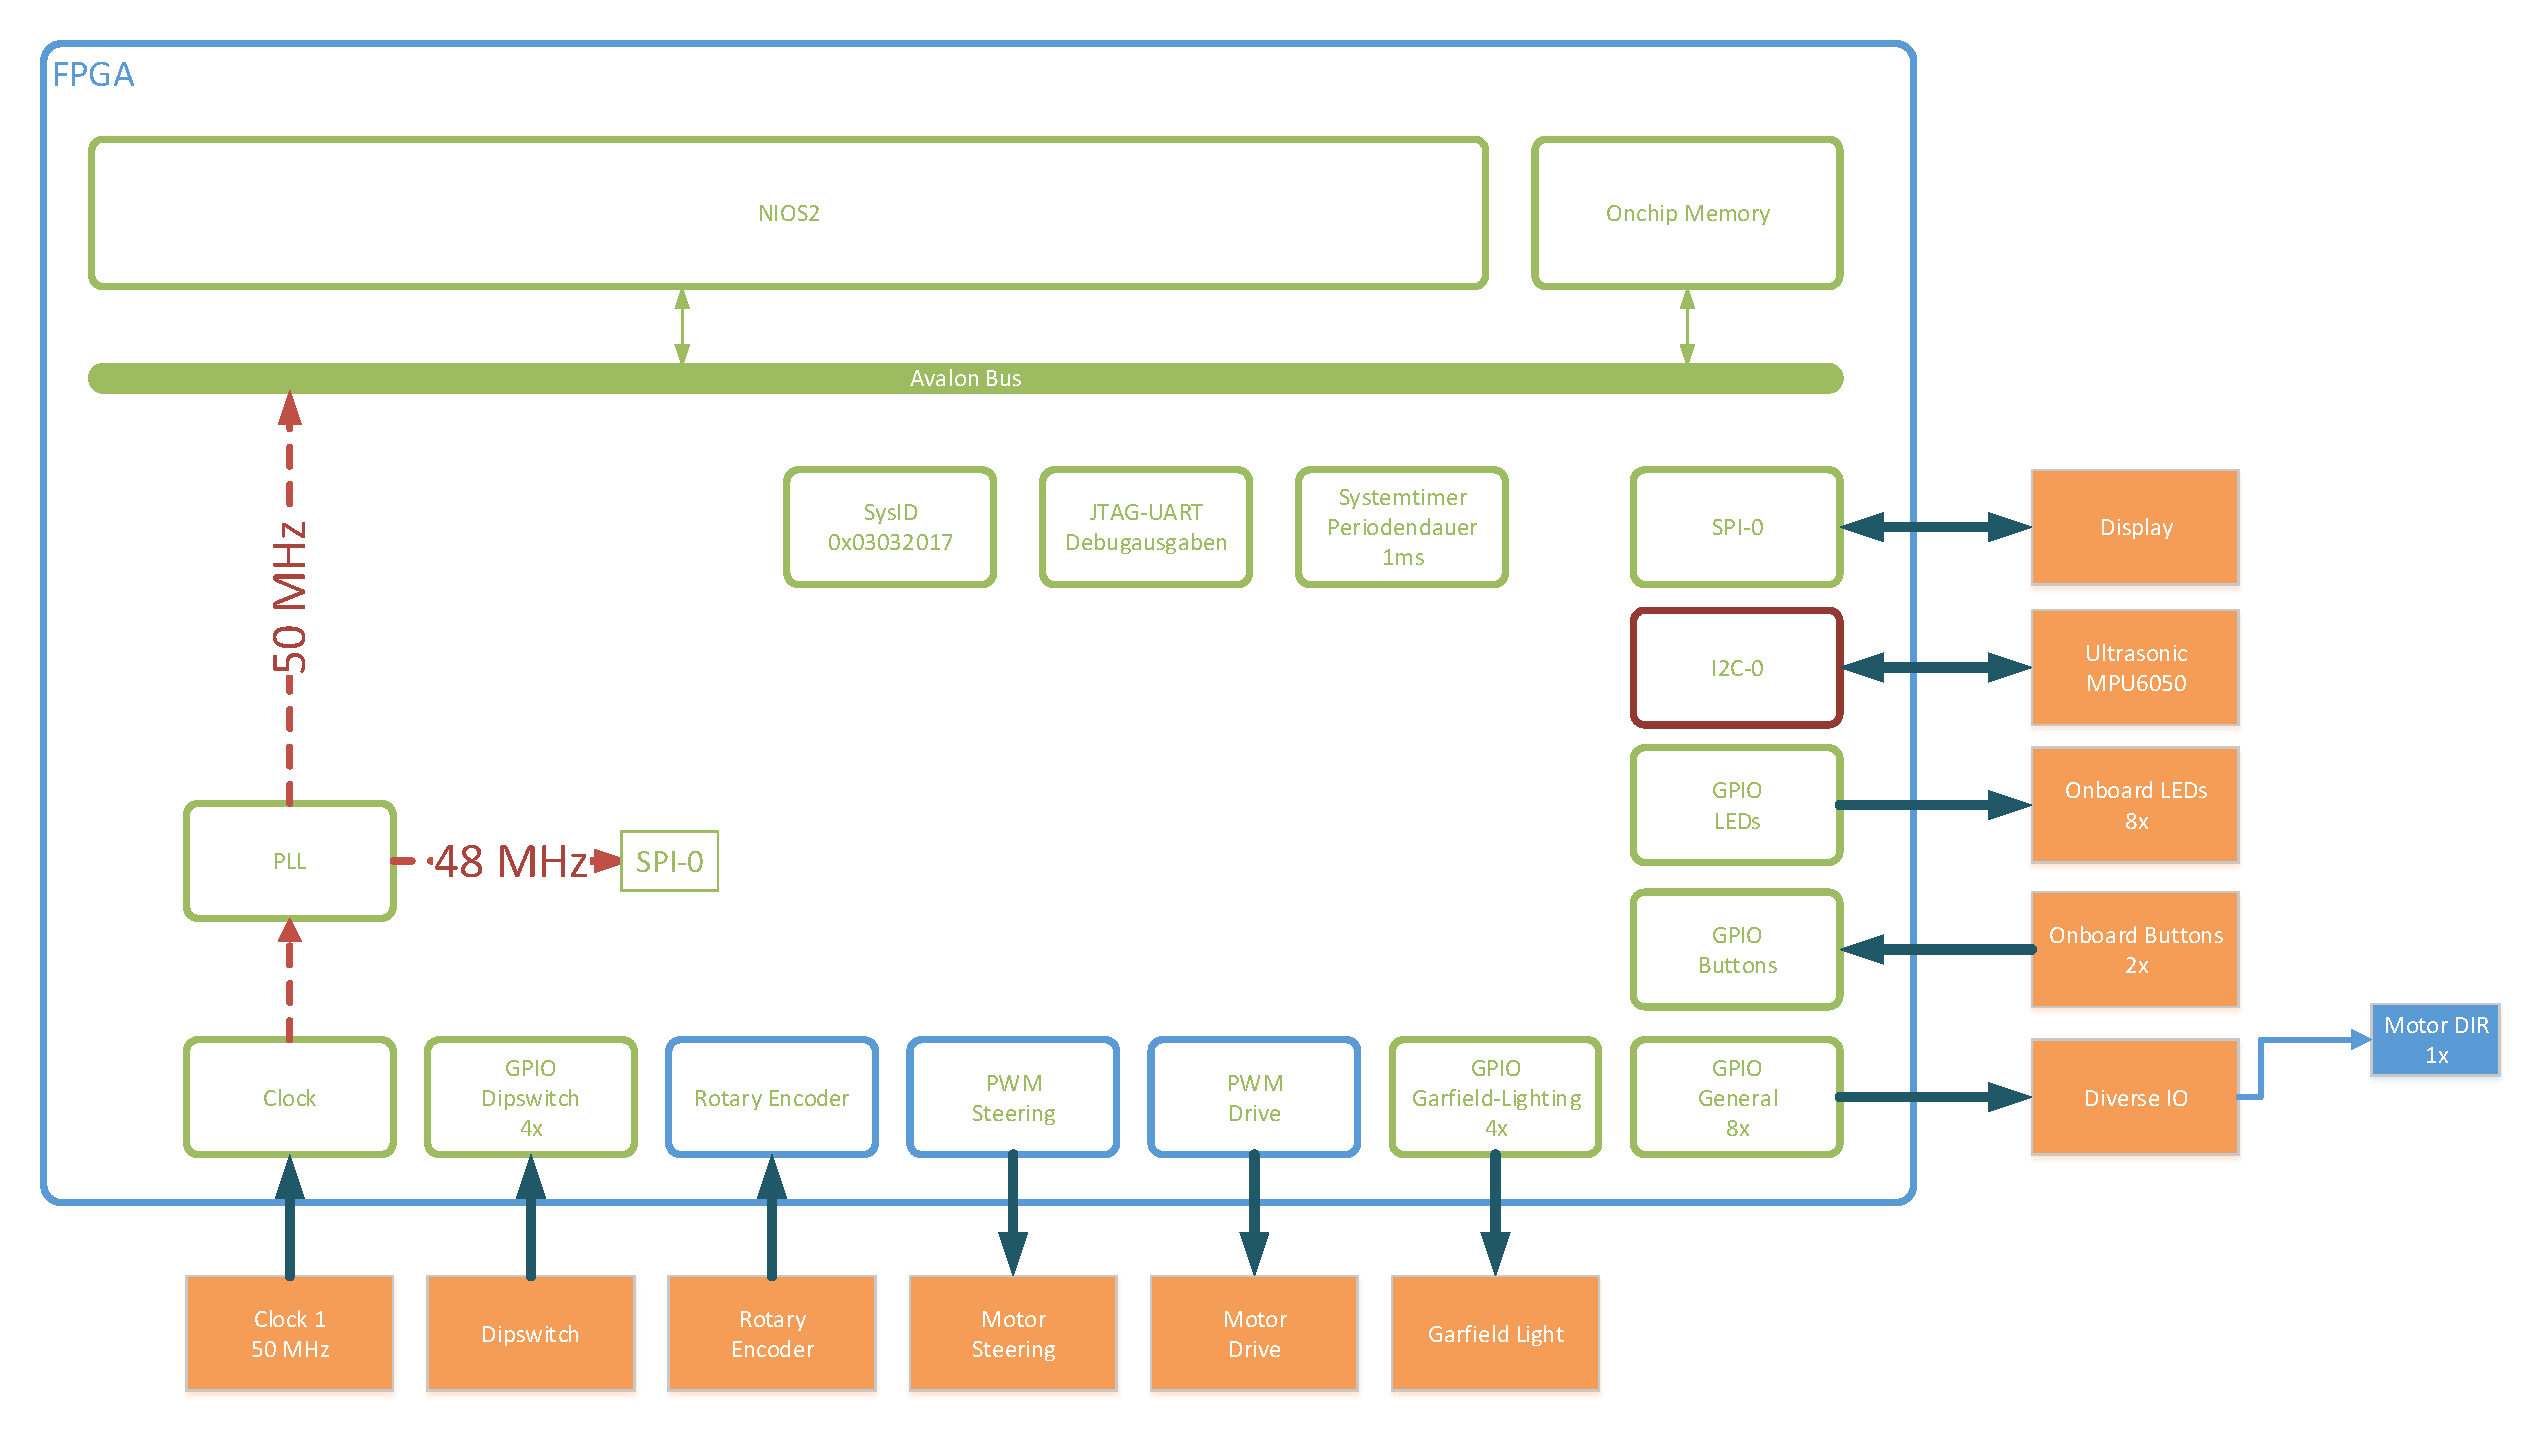
\includegraphics[angle=90, height=0.9\textheight]{Abb/Garfield_FPGA_Design_only_FPGA.pdf}
	\caption{Übersicht der (meisten) eingesetzten \ac{IP}-Cores. Die Abbildung verzichtet auf die Darstellung der Teile, die für die Kommunikation mit dem \ac{HPS} zuständig sind. Blau umrandet sind Cores, die im Rahmen des Projekts selbst progammiert wurden, grün diejenigen, die Teil der Altera Toolchain sind und rot externe IP-Cores von opencores.org}
	\label{FPGA_IP_FPGA_only}
\end{figure}

Abbildung \ref{FPGA_IP_FPGA_only} zeigt eine Übersicht der eingesetzten \ac{IP}-Cores und deren Verbindung zur Außenwelt. Ausgenommen sind die \ac{IP}-Cores, die für die Kommunikation mit dem \ac{HPS} benötigt werden. Die nachfolgende Tabelle beschreibt die Funktion der einzelnen IP-Cores im Detail und Besonderheiten dazu.

\begin{longtable}[ht]{|p{0.1\textwidth} | p{0.9\textwidth} |}
	\hline
	\textbf{Name} & \textbf{Beschreibung}\\
	\hline
	SPI-0 & Stellt einen SPI-Datenbus mit 24MHz Clock-Frequenz zur Verfügung. Es werden insgesamt 3 Chipselect Signale zur Verfügung gestellt, wobei aktuell nur eines für das Display benutzt wird. In der aktuellen Ausbaustufe wird nur das Display auf dem Arduino-Header auf dem FPGA angesteuert.\\ \hline
	I2C-0 & Stellt einen I2C Datenbus zur Verfügung. Der \ac{IP}-Core stammt von \href{opencores.org}{opencores.org} und wurde manuell integriert. Er stellt u.a. eine eine in Software änderbare Clock-Frequenz zur Verfügung und bindet die Ultraschallsensoren und die MPU-6050 an das System an.\\ \hline
	GPIO-X & Die verschiedenen GPIO Cores dienen dazu einfache Peripherie anzubinden. Dazu gehören die LEDs, die Dip-Switches, die Buttons und generische IOs, die im Projekt benötigt werden um z.B. die Drehrichtung des Motors einzustellen. \\ \hline
	PWM X & Die beiden PWM \ac{IP}-Cores erzeugen Signale zur Geschwindigkeitssteuerung und für den Lenkmotor. \\ \hline
	Rotary-Encoder & Der Rotary Encoder zählt die steigenden Flanken der NAME. Durch Abfragen des Ergebnisregisters in regelmäßigen festen Zeitinervallen kann die aktuelle Geschwindigkeit, die an den Rädern anliegt, gemessen werden. Leider funktioniert der NAME aktuell nicht mehr. Um das Signal zu nutzen müsste man die Hardware neu aufbauen bzw. ersetzen.\\ \hline
	Clock \& \ac{PLL} & Die externe Referenzclock taktet mit 50 MHz. Dieses Signal wird über eine \ac{PLL} allen beteiligten IP-Cores bereitgestellt. Auch die \ac{FPGA}-\ac{HPS} Bridges werden mit dem 50MHz Signal gespeist. Einzige Ausnahme bildet der SPI-0 Core. Um eine Frequenz von 24MHz zu erreichen (die maximale Frequenz mit der das Display angesprochen werden darf) wird ein vielfaches dieser Frequenz benötigt. Das nächsthöhere verfügbare vielfache der 24MHz sind 48MHz. Die selbst geschriebenen \ac{IP}-Cores sind von der Frequenz der \ac{PLL} abhängig. Erhöht man die Frequenz der \ac{PLL} auf z.B. 100MHz um mehr Laufzeit für einzelne Funktionen zur Verfügung zu haben, muss man die Frequenz in den \ac{IP}-Cores manuell anpassen! \\ \hline
	SysID & Mit der System ID (in Kombination mit einem Zeitstempel) kann man das Hardware Design eindeutig identifizieren. Dies ist hilfreich wenn mehrere Hardware- und Softwareversionen existieren, die parallel entwickelt werden. Um Zugriffsfehler auf Register oder ähnliches zu vermeiden, kann die Software die System-ID nutzen um Funktionen ab- bzw. zuzuschalten. \\ \hline
	JTAG-UART & Mit Hilfe dieses Cores kann man printf ähnliche Ausgaben für Debug-Ausgaben an einen angesteckten PC schicken. \\ \hline
	Systemtimer & Der Systemtimer ist ein kontinuierlich laufender Timer, der sich alle 1ms automatisch erhöht. Außerdem erzeugt er ein Interrupt, das FreeRTOS zur internen Zeitbestimmung nutzt. \\ \hline
	NIOS2 & Hierbei handelt es sich um eine Softcore-CPU. Diese wird von Altera zur Verfügung gestellt (inkl. Toolchain) und kann unbegrenzt benutzt werden (mit entsprechender Lizenz). Es handelt sich um eine 32-bit \ac{RISC} Architektur die durchaus eine weite Verbreitung im industriellen Umfeld genießt. Weiter Informationen dazu findet man unter \href{https://www.altera.com/products/processors/overview.html}{https://www.altera.com/products/processors/overview.html} \\ \hline
	Onchip Memory & Ein einfacher \ac{IP}-Core, der Speicherbausteine auf dem \ac{FPGA} nutzt um RAM(hier genutzt) oder ROM (nicht genutzt) zu erzeugen. Dieser Speicher kann dann von einem Prozessor (hier der NIOS2) als Instruktions- und Datenspeicher genutzt werden. In der aktuellen Ausbaustufe ist die Speichergröße mit 128kB angegeben. \\ \hline
\end{longtable}
\todo{NAME}

\begin{figure}
	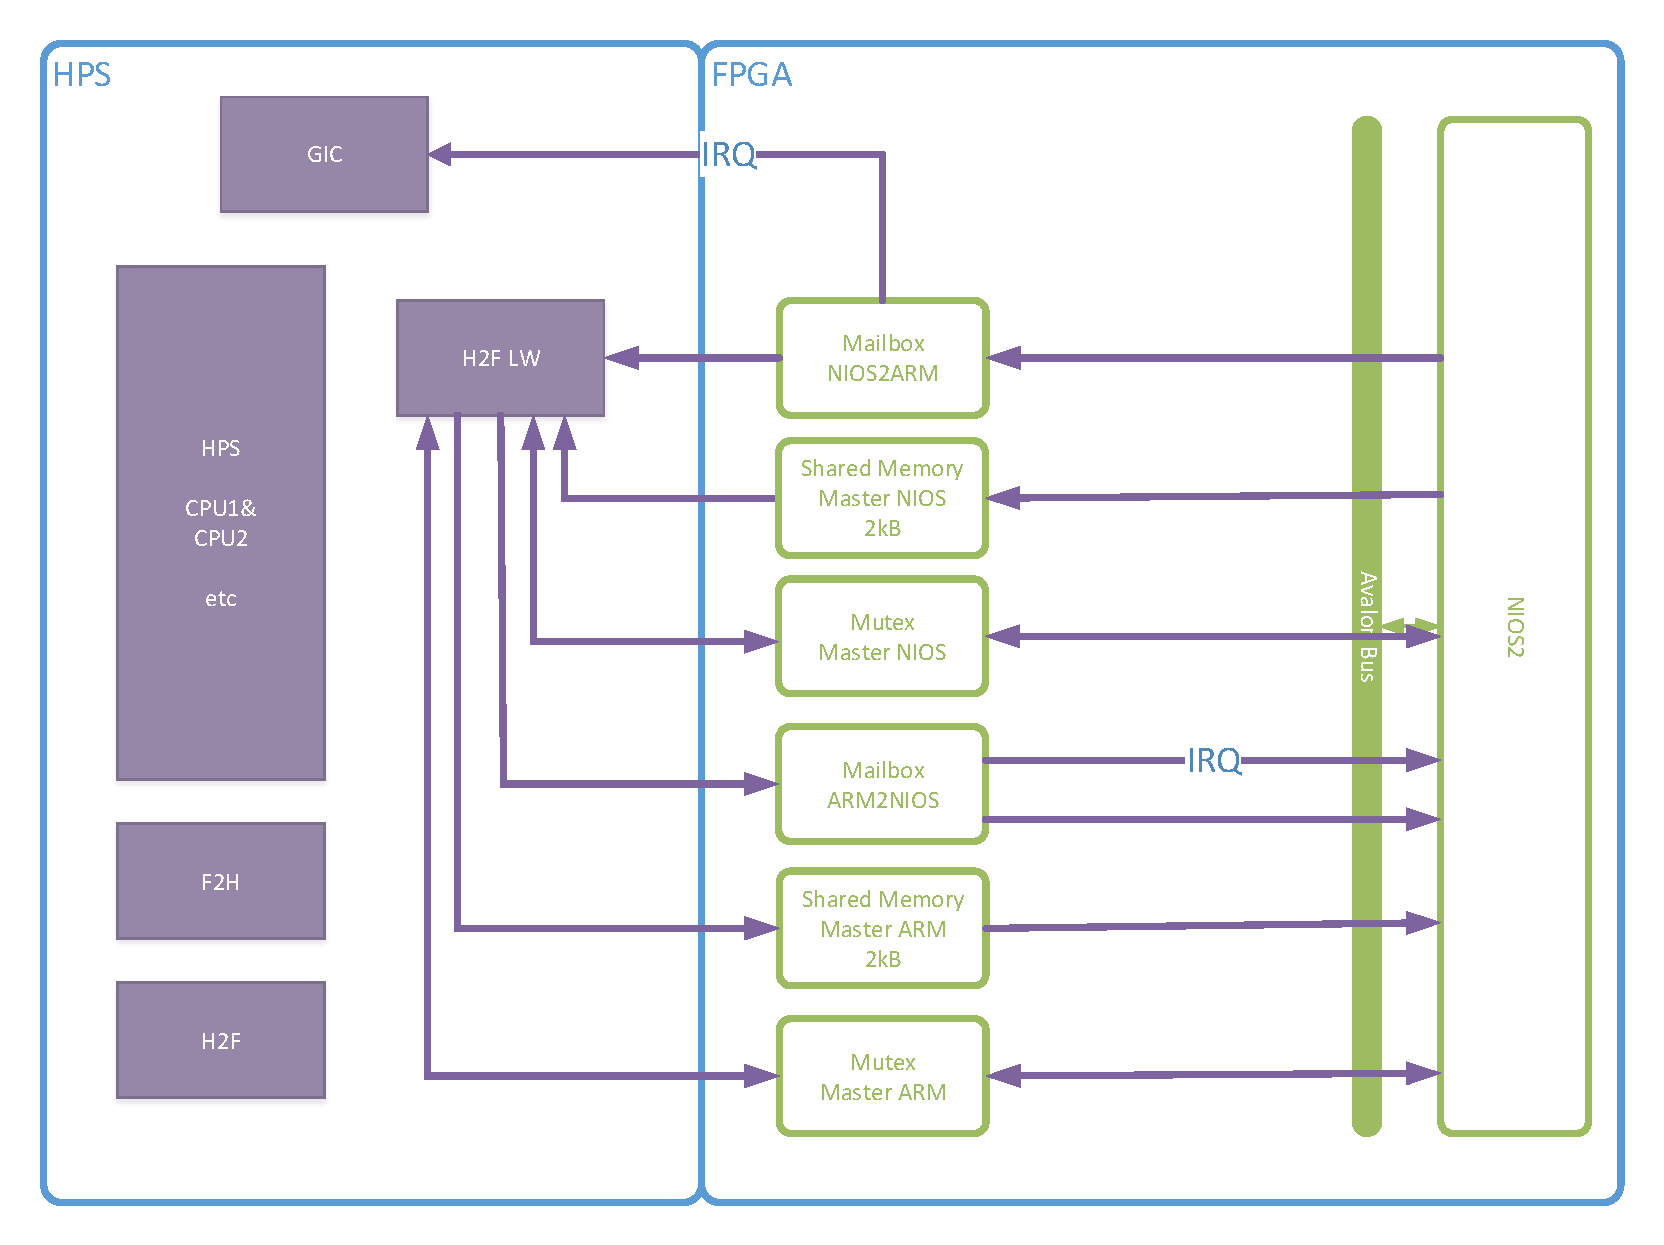
\includegraphics[angle=0, width=\textwidth]{Abb/Garfield_FPGA_Design_comm.pdf}
	\caption{\ac{IP}-Cores und deren Kontrollfluss, die an der Kommunikation zwischen NIOS2 und \ac{HPS} beteiligt sind.}
	\label{FPGA_IP_FPGA_comm}
\end{figure}

Abbildung \ref{FPGA_IP_FPGA_comm} zeigt die \ac{IP}-Cores, die für die Kommunikation zwischen \ac{FPGA} und \ac{HPS} benötigt/eingesetzt werden. Auf der linken Seite der Abbildung ist das \ac{HPS} System illustriert. Auf dieser Seite sind im wesentlichen drei Hardwareeinheiten an der Kommunikation beteiligt:
\begin{itemize}
	\item GIC - Der ARM \textit{General Interrupt Controller} : Dieser Controller ist ein sehr mächtiger Interrupt Controller, der u.a. die Interruptverarbeitung an die einzelnen CPUs verteilt. Insgesamt stehen 64 Interrupts zur Verfügung, die aus dem \ac{FPGA} heraus ausgelöst werden können. Auf dem eingesetzten Cyclone V beginnen diese mit der Interrupt ID 72 vom GIC. Genauere Informationen zum GIC kann man entweder auf der Homepage von ARM oder \cite{Using_GIC} erhalten.
	\item H2F LW - Die \ac{HPS}2\ac{FPGA} Leightweight Bridge : Dies ist eine der drei Bridges, mit denen zwischen \ac{FPGA} und \ac{HPS} kommuniziert werden kann. Dies ist keine High-Performance Bridge, es ist aber keine großen Änderungen notwendig, das System auf eine der anderen Bridges umzubauen. Diese Bridge \textbf{muss} aktiviert werden, bevor über sie kommuniziert werden kann. Ist die Bridge nicht aktiviert, treten \textit{Segmentation Faults} auf (kein gültiger Speicherbereich). Im Prinzip befindet sich \textquotedblleft hinter\textquotedblright der Bridge ein Speicherbereich, der durchgehend addressiert werden kann um direkt in Register zu schreiben. Auch lesende Zugriffe daraus können erfolgen \cite{FPGA_Workshop}.
	\item CPUs - Die ARM A9 Applikationsprozessoren dienen zur Verarbeitung der Interrupts bzw. zum triggern der einzelnen IP-Cores.
\end{itemize}

Es folgt eine Beschreibung der \ac{IP}-Cores, die für die Kommunikation gebraucht werden. Da die Kommunikationseinheiten in beide Richtungen analog aufgebaut sind, beschränkt sich die Beschreibung auf einen Teil:
\begin{itemize}
	\item Mailbox X2Y : Die Mailbox ist ein einfacher IP-Core der Nachrichten von einem Buspartner (X, z.B. NIOS2) einem anderen Buspartner (Y, z.B. ARM) zur Verfügung stellt. Es gibt also einen Transmitter und einen Receiver. Beide sind über eigene Interfaces (und damit über ihren eigenen Addressbereich) an die Mailbox angeschlossen. Die Nachrichtenübermittlung erfolgt mit Hilfe von zwei Registern:
	\begin{itemize}
		\item Command Register - Dieses Register kann vom Empfänger nur gelesen werden. Es dient dazu, ein Kommando oder Nachricht an den Empfänger zu senden. Ein schreibender Zugriff auf dieses Register vom Sender löst das zugehörige Interrupt aus, dass vom Empfänger verarbeitet werden muss.
		\item Pointer Register - In diesem Register wird die Addresse, in der die eigentliche Nachricht im Speicher steht, übertragen. Sollen nur ganz kleine Nachrichten (4 oder 8 Bytes) übertragen werden, kann man das Pointer und Command Register dazu benutzen, die Nachricht zu übertragen. In diesem Projekt wird aber die eigentliche Nachricht im Shared Memory übertragen, in der Mailbox nur die Addresse im Shared Memory und ein Kommando im Command Register
	\end{itemize}
	Eine detailierte Beschreibung des Cores findet sich unter \cite[470ff]{embedded_guide}
	\item Shared Memory Master X - Dieser Speicher, der wie der Arbeitsspeicher des NIOS2 direkt im \ac{FPGA} synthetisiert wird, dient der Nachrichtenübermittlung. Dort werden die Nutzdaten einer Nachricht von X reingeschrieben und können zu einem späteren Zeitpunkt vom Empfänger Y ausgelesen werden. Es wurde sich bewusst dazu entschieden zwei Shared Memory zu benutzen um eine jegliche Kollision zu vermeiden bzw. zu vereinfachen. Die Größe beider Speicherbereiche beträgt jeweils 2kB. Dies reicht für die aktuellen Nachrichten leicht aus. Zu einem späteren Zeitpunkt können die Bereiche auch noch vergrößert werden, sollte der Speicher nicht groß genug sein Nachrichten zu übertragen.
	\item Mutex Master X - Dies ist ein spezieller \ac{IP}-Core, der auch als Teil des Altera \ac{IP}-Core Katalogs zur Verfügung stellt. Dieser hat nur ein Register, das hier betrachtet werden soll und erlaubt einen atomaren Mutex Zugriff auf geteilte Resourcen. Die geteilte Resource, die über diesen Mutex gesperrt wird ist der zugehöriger Shared-Memory. Die Referenz für diesen Core ist ebenfalls \cite[319ff]{embedded_guide}. Das Register besteht aus zwei Teilen: die oberen 16 Bit werden als Speicherplatz für die CPU-ID (der NIOS2 hat die ID 0x03, der ARM immer 0x01) benutzt. In die unteren 16 Bit kann ein beliebiger Wert gespeichert werden. Ein lesender Zugriff auf den Mutex ist immer möglich. Ein schreibender Zugrif ist nur möglich wenn
	\begin{itemize}
		\item Die CPU-ID mit der CPU-ID übereinstimmt, dessen Wert man in das Register schreiben will.
		\item (oder) Der Wert (untere 16-Bit) Null ist.
	\end{itemize}
	Man kann also nur schreibend auf den Mutex zugreifen, wenn einem der Mutex bereits gehört oder der Mutex frei (=0) ist. Nach einem schreibenden Zugriff muss der Registerwert mit dem Wert der geschrieben wurde verglichen werden. Stimmen beide Werte überein, hat der Schreiber den Mutex gelockt, andernfalls ist der atomare Lock fehlgeschlagen.
\end{itemize}

\section{Address-Map}

\begin{figure}
	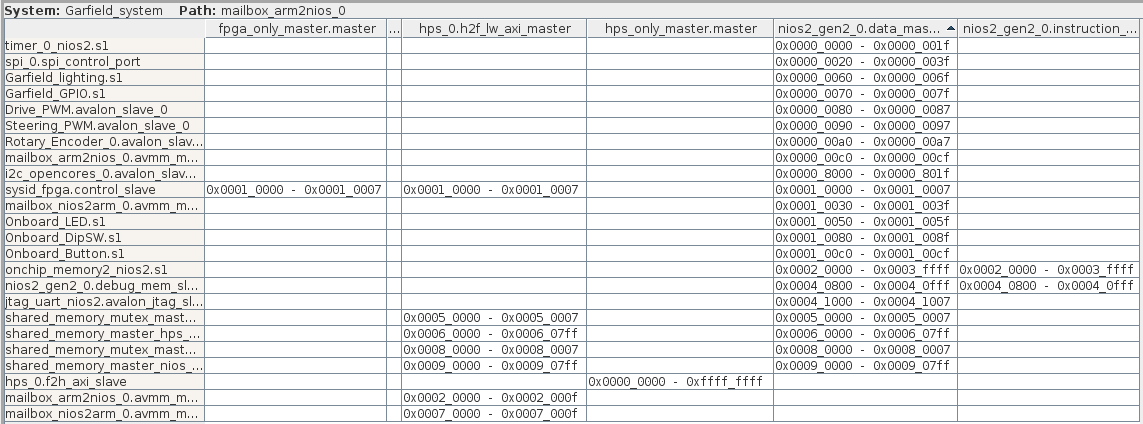
\includegraphics[width=\textwidth]{Abb/Address_Map.png}
	\caption{Übersicht über die Addressen und Addressbereiche im System}
	\label{FPGA:AddrMap}
\end{figure}

Abbildung \ref{FPGA:AddrMap} zeigt die Addressen die im System benutzt werden und den zugehörigen Addressbereich der verfügbar ist. Diese Addressmap ist auch im QSYS-Projekt des Projektes verfügbar.

\section{Eigenentwickelte \ac{IP}-Cores}

\subsection{Der PWM-Generator} generiert ein PWM Signal auf die Ausgabeleitung. Der Registerzugriff ist in Tabelle \ref{hw:pwm} dargestellt

\begin{table}
\begin{longtable}[]{@{}c|l|c|c|l@{}}
	\textbf{Bit} & \textbf{Name} & \textbf{Access} & \textbf{Reset Value} &
	\textbf{Description}\tabularnewline

	\endhead
	\texttt{7\ ...\ 0} & control & RW & 0 & sets the dutycylce of the PWM
	signal generator\tabularnewline
	\texttt{31\ ...\ 7} & - & R & 0 & not used\tabularnewline

\end{longtable}
\caption{Registermap des PWM Cores}
\label{hw:pwm}
\end{table}

\subsection{Der Rotary Encoder} \ac{IP}-Core kann steigende Flanken von einer externen Flanke zählen, hat ein auslesbares Ergebnisregister (siehe \ref{hw:rotary:result})und ein Controlregister (siehe \ref{hw:rotary:control}).

\begin{table}
\begin{longtable}[]{@{}clccl@{}}
	\begin{minipage}[b]{0.13\columnwidth}\centering\strut
		\textbf{Bit}\strut
		\end{minipage} & \begin{minipage}[b]{0.08\columnwidth}\raggedright\strut
		\textbf{Name}\strut
		\end{minipage} & \begin{minipage}[b]{0.12\columnwidth}\centering\strut
		\textbf{Access}\strut
		\end{minipage} & \begin{minipage}[b]{0.17\columnwidth}\centering\strut
		\textbf{Reset Value}\strut
		\end{minipage} & \begin{minipage}[b]{0.15\columnwidth}\raggedright\strut
		\textbf{Description}\strut
		\end{minipage}\tabularnewline
		\endhead
		\begin{minipage}[t]{0.13\columnwidth}\centering\strut
			\texttt{0}\strut
			\end{minipage} & \begin{minipage}[t]{0.08\columnwidth}\raggedright\strut
			enable\strut
			\end{minipage} & \begin{minipage}[t]{0.12\columnwidth}\centering\strut
			RW\strut
			\end{minipage} & \begin{minipage}[t]{0.17\columnwidth}\centering\strut
			0\strut
			\end{minipage} & \begin{minipage}[t]{0.15\columnwidth}\raggedright\strut
			Enable bit for the core\strut
			\end{minipage}\tabularnewline
			\begin{minipage}[t]{0.13\columnwidth}\centering\strut
				\texttt{1}\strut
				\end{minipage} & \begin{minipage}[t]{0.08\columnwidth}\raggedright\strut
				clear\strut
				\end{minipage} & \begin{minipage}[t]{0.12\columnwidth}\centering\strut
				W\strut
				\end{minipage} & \begin{minipage}[t]{0.17\columnwidth}\centering\strut
				0\strut
				\end{minipage} & \begin{minipage}[t]{0.15\columnwidth}\raggedright\strut
				Clear bit. clears the result register and set it to 0; Must not be
				manually set to 0 after clearing. With the next rising edge of the clock
				it goes down on itself.\strut
				\end{minipage}\tabularnewline
				\begin{minipage}[t]{0.13\columnwidth}\centering\strut
					\texttt{2}\strut
					\end{minipage} & \begin{minipage}[t]{0.08\columnwidth}\raggedright\strut
					reset\strut
					\end{minipage} & \begin{minipage}[t]{0.12\columnwidth}\centering\strut
					W\strut
					\end{minipage} & \begin{minipage}[t]{0.17\columnwidth}\centering\strut
					0\strut
					\end{minipage} & \begin{minipage}[t]{0.15\columnwidth}\raggedright\strut
					Resets the whole core and set all values to default. At a read
					operation, it is always 0\strut
					\end{minipage}\tabularnewline
					\begin{minipage}[t]{0.13\columnwidth}\centering\strut
						\texttt{15\ ...\ 3}\strut
						\end{minipage} & \begin{minipage}[t]{0.08\columnwidth}\raggedright\strut
						not accessable\strut
						\end{minipage} & \begin{minipage}[t]{0.12\columnwidth}\centering\strut
						-\strut
						\end{minipage} & \begin{minipage}[t]{0.17\columnwidth}\centering\strut
						0\strut
						\end{minipage} & \begin{minipage}[t]{0.15\columnwidth}\raggedright\strut
						-\strut
						\end{minipage}\tabularnewline
						\begin{minipage}[t]{0.13\columnwidth}\centering\strut
							\texttt{16}\strut
							\end{minipage} & \begin{minipage}[t]{0.08\columnwidth}\raggedright\strut
							error\strut
							\end{minipage} & \begin{minipage}[t]{0.12\columnwidth}\centering\strut
							R\strut
							\end{minipage} & \begin{minipage}[t]{0.17\columnwidth}\centering\strut
							0\strut
							\end{minipage} & \begin{minipage}[t]{0.15\columnwidth}\raggedright\strut
							Indicates an error within the counting process. You should reset the
							core!\strut
							\end{minipage}\tabularnewline
							\begin{minipage}[t]{0.13\columnwidth}\centering\strut
								\texttt{31\ ...\ 17}\strut
								\end{minipage} & \begin{minipage}[t]{0.08\columnwidth}\raggedright\strut
								not accessable\strut
								\end{minipage} & \begin{minipage}[t]{0.12\columnwidth}\centering\strut
								-\strut
								\end{minipage} & \begin{minipage}[t]{0.17\columnwidth}\centering\strut
								0\strut
								\end{minipage} & \begin{minipage}[t]{0.15\columnwidth}\raggedright\strut
								-\strut
								\end{minipage}\tabularnewline

\end{longtable}
\caption{Registermap des Controlregisters des Rotary Encoder}
\label{hw:rotary:control}
\end{table}

\begin{table}
	\begin{longtable}[]{@{}clccl@{}}
		\textbf{Bit} & \textbf{Name} & \textbf{Access} & \textbf{Reset Value} &
		\textbf{Description}\tabularnewline
		\endhead
		\texttt{31\ ...\ 0} & result & R & 0 & Result of the counting
		process\tabularnewline
	\end{longtable}
	\caption{Registermap des Ergebnisregisters des Rotary Encoder}
	\label{hw:rotary:result}
\end{table}
